% Sections 2, 3, and 4: Toolchain, Dataset & LTL Alignment, STAR Framework, and WebUI/SMV Infrastructure

\section{Execution Environment, Toolchain, and Controlled Setup}

\subsection{Software Toolchain and Runtime Isolation}
All compilation and functional test runs execute against a real Windows installation of \code{CODESYS Development System 3.5.22.40} (\code{CODESYS V3.5 SP22 Patch 4}) driven via its embedded IronPython~2.7 Scripting Engine, with \code{CODESYS Static Analysis Light} active. Candidate function blocks are built inside copies of a hash-frozen template project (\pathcode{codesys/templates/benchmark.project}, device target \code{Control Win V3 x64}, \code{template_sha256}: \texttt{\small\seqsplit{70d40be7b4b9bdf4a22619a7ba47156422cf6beaec692480f0e5ee2acbda8909}}). Runtime functional evaluation drives the compiled \code{FB_Task} under a \code{1ms} cyclic \code{ScriptTaskObject} running a generated \code{PLC_PRG} harness over the local simulation target; no external physical PLC hardware is connected.

Formal verification is dispatched dynamically across two symbolic model checkers: \textbf{NuSMV~2.7.1} (BDD engine) for pure Boolean and bounded integer controllers, and \textbf{nuXmv} (with the \code{MathSAT} SMT backend, default BMC depth 25) for designs containing IEEE-754 floating-point ports (\code{REAL}/\code{LREAL}) or unbounded arithmetic. Software orchestration and offline regression suites run on Python~3.12+ inside a standard environment, while real CODESYS compilation and gateway-connected simulation run inside normal un-sandboxed Windows processes because restricted sandboxes block APInstaller event-log writes and gateway communication.

\subsection{Experimental Matrix and Reasoning Configuration}
Following \pathcode{configs/fullflow_matrix.json}, evaluation uses a crossed $2 \times 2$ design across two frameworks---the self-developed \textbf{STAR} harness (\pathcode{self_harness}) and unmodified official \textbf{Codex CLI~v0.142.5}---and two foundation models accessible through the project relay (\pathcode{deepseek-v4.1-flash-1017} and \pathcode{gpt-6.1-terra}), totaling 128 planned task runs across 32 benchmark tasks (Table~\ref{tab:matrix}). Crucially, \textbf{all four conditions uniformly enforce maximum reasoning strength} (\code{reasoning.effort = "high"} in every API payload), isolating architectural and model differences without varying inference effort. Pre-configured ablation modes (\code{no_planner}, \code{no_dialect}, \code{no_selftest}) are additionally preserved in \pathcode{configs/experiments.json} for follow-up attribution studies.

\begin{table}[htbp]
\centering
\caption{Controlled $2 \times 2$ benchmark matrix spanning agent frameworks and foundation models.}
\label{tab:matrix}
\footnotesize
\begin{tabularx}{\textwidth}{@{}llL{0.28\textwidth}Y@{}}
\toprule
\textbf{ID} & \textbf{Agent Framework} & \textbf{Model Route} & \textbf{Reasoning Effort \& Runtime Transport} \\
\midrule
\textbf{E1} & \textbf{Codex CLI (\code{v0.142.5})} & \pathcode{deepseek-v4.1-flash-1017} & Max (\code{reasoning.effort = "high"}), local \code{CodexTransport} HTTP relay + MCP server \\
\textbf{E2} & \textbf{Codex CLI (\code{v0.142.5})} & \pathcode{gpt-6.1-terra} & Max (\code{reasoning.effort = "high"}), local \code{CodexTransport} HTTP relay + MCP server \\
\textbf{E3} & \textbf{STAR (\code{self_harness})} & \pathcode{deepseek-v4.1-flash-1017} & Max (\code{reasoning.effort = "high"}), native multi-stage \code{ResponsesClient} \\
\textbf{E4} & \textbf{STAR (\code{self_harness})} & \pathcode{gpt-6.1-terra} & Max (\code{reasoning.effort = "high"}), native multi-stage \code{ResponsesClient} \\
\bottomrule
\end{tabularx}
\end{table}

\subsection{Shared Budgets, Quotas, and Engineering Guardrails}
Rather than treating operational limits as optimal universal constants, runtime quotas act as symmetric guardrails for fairness and cost containment across agents. As logged in each 14~November~2026 run's \pathcode{generation/runtime_config.json}:
\begin{itemize}
  \item \textbf{Symmetric Tool and Call Quotas}: Each task allows at most \code{max_repairs = 2} compile-repair iterations (initial draft plus up to 2 repairs, i.e., $\le 3$ builds), \code{max_verifications = 3} formal checks (capped at \code{60s} each), \code{max_simulations = 3} internal self-test simulation rounds, at most \code{9} LLM requests, and a cumulative \code{300,000}-token cap. For Codex CLI, standalone \pathcode{mcp_server.py} enforces identical tool counters and rejects excess calls with \code{isError: true}.
  \item \textbf{Timeouts, Output Caps, and Lock Budget Decoupling}: Per-task wall time was bounded at \code{task_timeout = 1800s} during the main campaign (raised to \code{2400s} by default in the latest codebase revision), with \code{compiler_timeout = 180s}, \code{llm_timeout = 420s}, single-turn output caps of \code{24,576} (Coder/Tester) and \code{32,768} (Planner/Repair) tokens, and a cumulative fee fuse of \code{reported_cost_stop_cny = 75}. Recent hardening further decoupled the shared CODESYS mutex wait budget (\code{compiler_lock_timeout = 960s}, dynamically extended for long-duration timed simulations) from the compiler execution timeout so concurrent workers waiting on the single-instance IDE do not trigger premature lock timeouts.
  \item \textbf{Baseline Context Adaptation (\code{codex_transport.py})}: Because Codex CLI injects its own system prompt and tool schemas, applying STAR's tighter input context cap causes immediate prompt truncation; the relay layer relaxes total input context clipping for Codex CLI while preserving identical output token limits, reasoning effort, tool quotas, and stop rules.
\end{itemize}

\section{Benchmark Dataset and Formal Specification Design}

\subsection{Provenance, Normalization, and Independent Review}
The frozen dataset release \code{normalized-20261114} (SHA-256: \texttt{\small\seqsplit{d305f96c2faaa87f60a24be90c00ad0b32153492e741b87547d132c591e0e9ee}}) contains \textbf{32 control tasks}:
\begin{enumerate}
  \item \textbf{20 Public Tasks (\code{PUB001}--\code{PUB020})}: Ten problems derive from the public course task pool (\code{PUB001}--\code{PUB010}) and ten from instructor supplementary tasks (\code{PUB011}--\code{PUB020}). Automated alignment (\pathcode{requirements/source_alignment.json}) against the original 25-page question bank (fingerprint \code{4ce56562...}) confirms a text sequence similarity of \code{1.0} and complete interface matching across all 20/20 problems. Ambiguities common in natural-language prompts (concurrent priority order, invalid input sanitization, out-of-bounds clamping, initial output defaults) are clarified additively via \code{scan_semantics}, \code{safety_priority}, \code{assumptions}, and \code{specification_contract} without modifying the verbatim English statements. All 32 tasks underwent bilingual human verification.
  \item \textbf{12 Self-Built Tasks (\code{SELF001}--\code{SELF012}, AI-Generated + Human Reviewed)}: Marked explicitly with provenance \code{independent_synthesis}, these tasks were authored through \textbf{AI-assisted generation followed by human review}. An AI assistant initially synthesized problem specs, boundary conditions, engineering \code{rationale}, and 7--12 fixed scan sequences covering multi-actuator interlocks, hysteresis tank control, alternating pump rotation, consecutive-scan qualification, bit-parity checks, and bounded fault retries while avoiding structural duplication of public tasks. Each candidate spec was exercised in Python against an independent reference transition model and then manually audited via a bilingual review view for disambiguation, initialization, priority resolution, recovery edges, and LTL alignment. This review establishes internal benchmark consistency and does not constitute formal IEC~61508 safety certification.
\end{enumerate}

\subsection{Industrial Control Semantics and Diversity Metrics}
The corpus enforces strict \code{FUNCTION_BLOCK FB_Task} ownership conventions separating read-only \code{VAR_INPUT}, \code{VAR_OUTPUT}, and caller-owned persistent \code{VAR_IN_OUT} references (e.g., multi-pump banks in \code{PUB007}, analog channels in \code{PUB008}, recipe structs in \code{PUB017}, generic FIFOs in \code{PUB018}). Timing coverage deliberately combines pure scan-counted discrete state machines across \code{SELF001}--\code{SELF012} (immune to host scheduling jitter) with 6 real-timer public problems (\code{PUB004}, \code{PUB005}, \code{PUB006}, \code{PUB010}, \code{PUB012}, \code{PUB013}) totaling 315 non-zero \code{dt_ms} scan intervals. Table~\ref{tab:dataset} and Figure~\ref{fig:dataset} summarize benchmark breadth across difficulty tiers, control patterns, IEC~61131-3 types, and test-trace scale.

\begin{table}[htbp]
\centering
\caption{Diversity profile of the normalized 32-task IEC~61131-3 benchmark (\code{normalized-20261114}).}
\label{tab:dataset}
\footnotesize
\begin{tabularx}{\textwidth}{@{}L{0.21\textwidth}L{0.48\textwidth}Y@{}}
\toprule
\textbf{Dimension} & \textbf{Measured Coverage} & \textbf{Representative Tasks} \\
\midrule
\textbf{Source \& Difficulty} & 32 tasks (20 \code{public}, 12 \code{self_built}); Easy 10 (6+4), Medium 14 (8+6), Hard 8 (6+2) & Easy: \code{PUB001}, \code{SELF001}; Med: \code{PUB008}, \code{SELF007}; Hard: \code{PUB015}--\code{020}, \code{SELF011}--\code{012} \\
\textbf{Control Taxonomy} & Step sequencers, multi-mode arbitration, edge bit-counting, debounced/accumulated timers, moving averages, pump alternation, string parsing, struct CRUD, generic FIFOs & \code{PUB002} (edges), \code{PUB009} (filter), \code{PUB013} (HVAC), \code{PUB017} (recipe), \code{PUB018} (FIFO), \code{PUB019} (arm) \\
\textbf{IEC~61131-3 Types} & 21 distinct type forms over 260 declared ports: 205 \code{BOOL} plus 55 non-Boolean ports across 16 type families (\code{REAL}~10, \code{USINT}~9, \code{WORD}/\code{TIME}/\code{ARRAY}/\code{INT}~4 ea., \code{DWORD}/\code{DINT}~3 ea., \code{LTIME}/\code{UINT}/\code{ARRAY[*]}/\code{LREAL}/\code{STRUCT}/\code{VARIANT}~2 ea., \code{STRING}/\code{UDINT}~1 ea.) & \code{PUB008}/\code{009} (\code{ARRAY[*]}), \code{PUB004} (\code{LTIME}), \code{PUB014} (\code{STRING}), \code{PUB017}/\code{018} (\code{VARIANT}) \\
\textbf{I/O \& Fixed Traces} & I/O span $1/1$ to $18/6$; \textbf{276 fixed cases / 2,994 scan steps} (public 177 cases / 2,230 scans; self-built 99 / 764); mean 8.63 cases \& 93.56 scans/task & Min I/O: \code{PUB014} ($1/1$); Max I/O: \code{PUB019} ($18/6$, 17 cases / 306 scans); Longest: \code{PUB009} (455 scans) \\
\bottomrule
\end{tabularx}
\end{table}

\begin{figure}[htbp]
  \centering
  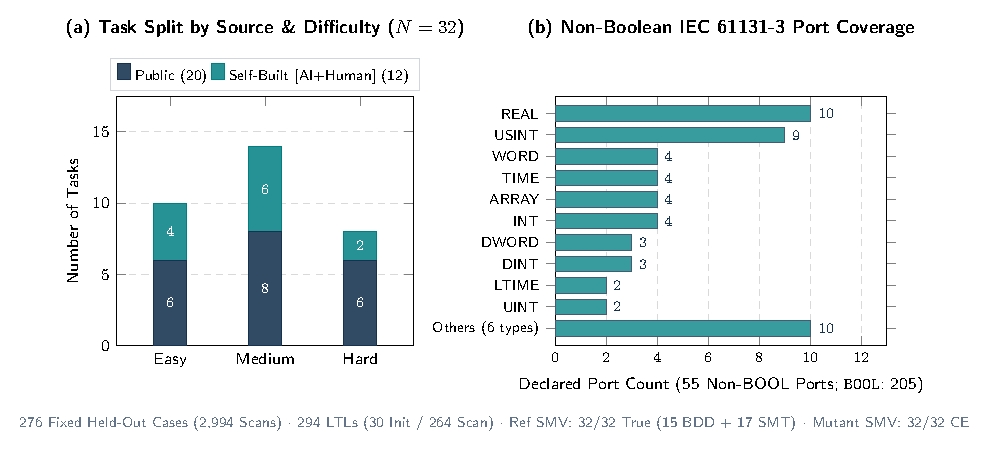
\includegraphics[width=0.98\textwidth]{fig1_dataset_composition.pdf}
  \caption{Dataset composition: (a)~stratified split across source and difficulty tiers ($N=32$); (b)~coverage of 55 non-Boolean IEC~61131-3 ports (excluding 205 \code{BOOL} ports) alongside aggregate trace and SMV dual-control counts.}
  \label{fig:dataset}
\end{figure}

\subsection{Scan-Aligned LTL Corpus and Dual-Control SMV Verification}
The benchmark incorporates \textbf{294 annotated LTL properties} (181 public, 113 self-built) partitioned strictly into two scopes:
\begin{itemize}
  \item \code{INITIAL_INSTANCE} \textbf{(30 formulas, task \code{P_init})}: Constraints checked prior to scan~0 immediately after function-block instantiation (e.g., outputs and retained latches initialized to \code{FALSE}), preventing erroneous application of temporal operator $\mathbf{G}$ across pre-execution states.
  \item \code{SCAN_SEQUENCE} \textbf{(264 formulas)}: Encompasses 50 explicit \code{safety} invariants, transition dynamics, persistent fault latching (expressed via weak-until expansions such as $\mathbf{G}\,Fault \lor (Fault\ \mathbf{U}\ (\neg Jam \land Reset))$ in \code{SELF004} when operator resets may remain idle indefinitely), fairness-guarded conditional liveness, and \code{CompleteBehavior} specifications.
\end{itemize}

Whereas Pre-Scan Moore conventions record outputs on the next cycle ($q[k+1]$), real CODESYS cyclic recorders and this benchmark log \textbf{End-of-Scan Records}:
\begin{equation}
  T[k] = \big(I[k],\; q[k],\; O[k]\big), \qquad q[k+1] = \delta\big(q[k], I[k]\big),\quad O[k] = \lambda\big(q[k], I[k]\big).
\end{equation}
Because scan~$k$'s sampled output $O[k]$ reflects same-scan combinational overrides immediately, safety stop preemption writes cleanly without next-state delay as $\mathbf{G}\big((StopBtn \lor EStop) \rightarrow \neg Motor\big)$, while cross-scan retention references explicit pre-state propositions (e.g., \code{qRun}), keeping discrete runtime traces and SMV models semantically locked.

To verify both specification soundness and fault sensitivity, every task ships an explicit reference SMV model (\pathcode{models/*_reference.smv}) alongside an adversarial mutant SMV injecting realistic logical or timing bugs (\pathcode{models/*_mutant.smv}). Tracked under SHA-256 freshness guarantees by \pathcode{smv_status.py} in \pathcode{configs/smv_verification_status.json}, \textbf{32/32 reference models achieve \code{MODEL_PROPERTIES_TRUE}} (15 \code{NuSMV} BDD + 17 \code{nuXmv} SMT; 285/285 explicit reference properties verified), while \textbf{32/32 negative-control mutant models produce \code{COUNTEREXAMPLE}} (15 BDD + 17 SMT), plus 1 verified \code{complete} BDD model.

\section{The STAR Agent Framework and Supporting Infrastructure}

\subsection{Overview and Leak-Free Architecture}
STAR replaces unstructured free-form agent loops with an artifact-centric multi-stage pipeline operating strictly on a physically scrubbed \code{agent_view()} input (Figure~\ref{fig:arch}). Every benchmark task strips reference implementations, \code{tests}, \code{test_bindings}, \code{specification_contract}, and \code{CompleteBehavior} entries prior to exposing prompts to either STAR or Codex CLI, preserving symmetric zero-leakage conditions until offline evaluation in \pathcode{batch.py}.

\begin{figure}[htbp]
  \centering
  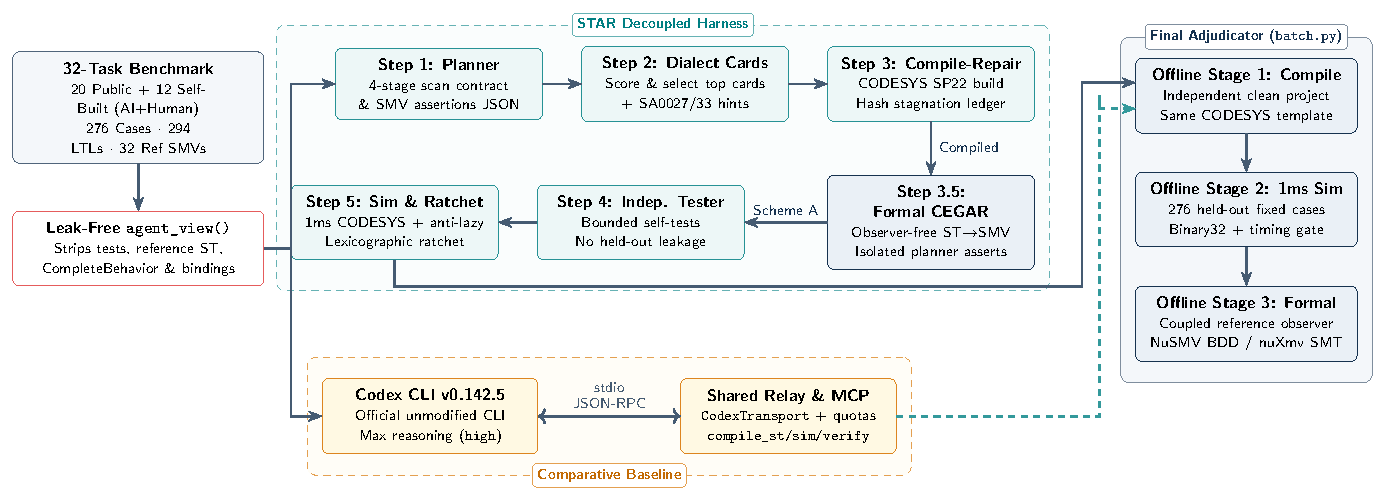
\includegraphics[width=\textwidth]{fig0_star_architecture.pdf}
  \caption{End-to-end architecture comparing the leak-free STAR decoupled pipeline, the symmetric \code{Codex CLI~v0.142.5 + MCP} baseline, and the three-stage offline adjudicator (\pathcode{batch.py}).}
  \label{fig:arch}
\end{figure}

\subsection{Core Design Elements and Engineering Trade-offs}
\begin{enumerate}
  \item \textbf{Task Organization (Step~1 Planner)}: Rather than mixing state-machine partitioning with low-level ST syntax in one generation turn, Step~1 emits a structured JSON scan blueprint specifying state enums, timer/edge instances with reset conditions, priority layers, initial values, and a four-phase deterministic scan skeleton: \code{1) input and edge sampling} $\rightarrow$ \code{2) safety preemption and state transitions} $\rightarrow$ \code{3) unconditional top-level TON/R_TRIG execution} $\rightarrow$ \code{4) post-state output assignment}. Step~3 guarantees timers never freeze inside skipped \code{CASE}/\code{IF} arms, while Steps~2 and~4 prevent intra-scan safety-override conflicts.
  \item \textbf{Context Management Trade-offs (\pathcode{task_view.py}, \pathcode{dialect_cards.py}, \pathcode{harness.py})}:
    \begin{itemize}
      \item \emph{Selective Dialect Cards}: Injecting the complete CODESYS manual wastes context budget and dilutes attention on control logic, whereas omitting dialect nuances invites repeated compiler faults. As a practical trade-off between guidance completeness and prompt focus, STAR curates 8 concise dialect cards (\code{VARIANT}, \code{ARRAY[*]}, \code{LTIME}, unconditional \code{TON}/\code{R_TRIG}, \code{VAR_IN_OUT} structs, 0-based \code{s[i]} vs.\ 1-based \code{STRING} library indexing, and pre-\code{CASE} mode normalization) alongside static-analysis hints, ranking them against interface/text cues and keeping the top-ranked subset (currently top~4).
      \item \emph{Diagnostic Compaction \& Stagnation Ledger}: \code{compact_diagnostics()} extracts localized code snippets and line/column pointers around compiler errors, attaches actionable advice for \code{SA0027} (keyword shadowing) and \code{SA0033} (unused declarations), and pairs with a bounded sliding-window failure log (\code{attempt_ledger}) to curb A$\leftrightarrow$B repair oscillation without unbounded prompt growth.
      \item \emph{First-Divergence Desensitized Feedback}: Both simulation and formal loops feed back only the minimal input prefix up to the first failing scan (\code{first_bad_step}) or shortest counterexample trace.
    \end{itemize}
  \item \textbf{Real Compiler Verification \& Five-Stage \code{ST->SMV} Engine (\pathcode{compiler.py}, \pathcode{st_verifier.py})}:
    \begin{itemize}
      \item \emph{CODESYS Rebuild \& \code{1ms} Replay}: Non-ASCII workspace paths are automatically relocated into ASCII staging directories, builds verify \code{app.generate_code()} static checks, nonces, and template SHA-256 digests, and simulation tests execute isolated \code{FB_Task} test programs via \code{binary32} byte-exact float matching to avoid JSON rounding drift.
      \item \emph{Observer-Free In-Loop Verification (Scheme~A) \& Expression Lowering}: Inside Step~3.5 (and baseline MCP \code{verify_st}), \code{st_verifier.py} parses ST ASTs into pre-init ($t=-1$) and single-scan SSA transition models ($t \ge 0$) with qualified enum resolution and built-in symbolic semantics for 9 standard FBs (\code{TON}, \code{TOF}, \code{TP}, \code{R_TRIG}, \code{F_TRIG}, \code{RS}, \code{SR}, \code{CTU}, \code{CTD}). Built-in \code{_SMVExprParser} and \code{_translate_st_ltl_to_smv} automatically normalize mixed Boolean/relational operators, unfold chained comparisons (e.g., \code{-4 <= x <= 4}), translate typed base literals (\texttt{\small DWORD\#0}, \texttt{\small WORD\#16\#...}), and reject malformed nested temporal expressions prior to invoking BDD/SMT solvers. Crucially, internal generation runs \code{Scheme A} without linking the held-out reference observer (\code{include_expected_observer=False}), while keeping Planner-generated \code{formal_assertions} isolated so malformed planner assertions automatically fall back to benchmark LTLs rather than halting verification. Only frozen final candidates enter Stage~3 coupled reference-observer equivalence checks. Unsupported constructs (e.g., \code{VARIANT}, \code{__VARINFO}) cleanly report \code{UNSUPPORTED_ST} alongside \code{PASS}, \code{COUNTEREXAMPLE}, \code{INCONCLUSIVE}, \code{TIMEOUT}, and \code{TOOL_ERROR}.
    \end{itemize}
  \item \textbf{Repair Loop Engineering Trade-offs \& Termination}:
    When Step~4 constructs self-tests without oracle ground truth, forbidding all test pruning risks misleading repairs from faulty self-tests, while unrestricted pruning risks trivializing tests. STAR enforces a structural constraint---\textbf{\code{lazy_rejection_blocked}}---disallowing case dismissal unless the candidate code hash substantively changes. Candidate acceptance follows a lexicographic 4-tuple \code{(compiled, formal_passed_props, sim_passed_cases, -len(rejected_case_ids))}: if a candidate edit regresses any higher-priority criterion, the ratchet rolls back to the best verified version. The trade-off is favoring reliable local convergence under tight repair budgets over multi-step disruptive refactoring. Finally, infrastructure faults (\code{TOOL_ERROR}, \code{TIMEOUT}, \code{UNVERIFIED}) remain cleanly separated from logical outcomes.
\end{enumerate}

\subsection{Specification Auditing Support and Zero-Dependency WebUI Visualization}
Beyond core synthesis, engineering effort invested substantially in making formal specifications auditable, regressions reproducible offline, and agent traces visually inspectable:

\subsubsection{Multi-Layer Specification Auditing and Offline Regression}
\begin{enumerate}
  \item \textbf{\code{ScanContract} Dual-Mode Offline Regression}: Combines transition-model multi-step contract validation and differential random testing so the core timing and semantic suite runs fast on headless Linux nodes without Windows/CODESYS dependencies.
  \item \textbf{Three-Variant SMV Freshness Tracking (\code{smv_status.py})}: Automatically discovers \code{reference}, \code{complete}, and \code{mutant} SMV files per task, infers \code{bdd} vs.\ \code{smt} solver requirements, probes \code{NuSMV}/\code{nuXmv} binary availability, and hashes model/config state into \pathcode{configs/smv_verification_status.json}, flagging edited artifacts automatically as \code{STALE} (or \code{CHECKER_MISSING}/\code{UNVERIFIED}) so outdated proofs are never reused.
  \item \textbf{Six-Category LTL Symbol Taxonomy (\code{symbol_glossary.py})}: Parses every identifier appearing inside LTL formulas and contracts and assigns it into six semantic classes---\code{input} ($I[k]$), \code{output} ($O[k]$), \code{persistent_inout} (caller-owned \code{VAR_IN_OUT}), \code{obs_history} (prior-scan output $O[k-1]$), \code{ghost_state} (cross-scan reference state, edge memory $I[k-1]$, timer internals), and \code{alias} (combinational/temporal/contract macro aliases)---paired with bilingual definitions to eliminate observer-variable ambiguity during audits.
\end{enumerate}

\subsubsection{Full-Stack Bilingual Industrial WebUI (\code{webui.py} \& \code{run_trace.py})}
Implemented strictly over Python standard-library HTTP services with zero third-party frontend/backend dependencies, the WebUI unifies live backend status diagnostics and four specialized workspaces:
\begin{enumerate}
  \item \textbf{Dataset \& Specs (\code{tab-explorer})}: Supports source/difficulty filtering across all 32 tasks, side-by-side bilingual spec inspection, nested-bracket LTL highlighting with click-to-inspect six-class definitions (\code{spec-popover} powered by \pathcode{symbol_glossary.py}), reference ST/\code{.smv} inspection, and live in-browser \code{NuSMV}/\code{nuXmv} re-verification via \pathcode{/api/check-reference-model}.
  \item \textbf{Agent Workflow (\code{tab-trace} + \pathcode{run_trace.py})}: Safely resolves workspace artifacts inside \pathcode{experiments/} and \pathcode{results/raw/} to reconstruct complete execution timelines---displaying Planner contract JSON, Dialect card selections, per-turn \code{version_*} syntax diffs, compact diagnostics, and CEGAR/simulation repair iterations.
  \item \textbf{Sandbox \& Waveform Lab (\code{tab-sandbox})}: Provides an interactive ST editor with live demo chips connected to \pathcode{/api/evaluate}, \pathcode{/api/verify-candidate}, and \pathcode{/api/export-verify}, plus \code{_build_step_waveforms()} to plot digital square waves and analog step trajectories while highlighting the exact \emph{first-divergence scan} where candidate behavior deviates from expected traces.
  \item \textbf{Benchmark Results (\code{tab-benchmark})}: Aggregates multi-condition experiment summaries via \pathcode{/api/experiments} across overall, public/self-built, and difficulty splits (corresponding directly to the aggregate metrics in Section~5.2).
\end{enumerate}
